% Options for packages loaded elsewhere
\PassOptionsToPackage{unicode}{hyperref}
\PassOptionsToPackage{hyphens}{url}
\PassOptionsToPackage{dvipsnames,svgnames*,x11names*}{xcolor}
%
\documentclass[
]{article}
\usepackage{amsmath,amssymb}
\usepackage{lmodern}
\usepackage{ifxetex,ifluatex}
\ifnum 0\ifxetex 1\fi\ifluatex 1\fi=0 % if pdftex
  \usepackage[T1]{fontenc}
  \usepackage[utf8]{inputenc}
  \usepackage{textcomp} % provide euro and other symbols
\else % if luatex or xetex
  \usepackage{unicode-math}
  \defaultfontfeatures{Scale=MatchLowercase}
  \defaultfontfeatures[\rmfamily]{Ligatures=TeX,Scale=1}
\fi
% Use upquote if available, for straight quotes in verbatim environments
\IfFileExists{upquote.sty}{\usepackage{upquote}}{}
\IfFileExists{microtype.sty}{% use microtype if available
  \usepackage[]{microtype}
  \UseMicrotypeSet[protrusion]{basicmath} % disable protrusion for tt fonts
}{}
\makeatletter
\@ifundefined{KOMAClassName}{% if non-KOMA class
  \IfFileExists{parskip.sty}{%
    \usepackage{parskip}
  }{% else
    \setlength{\parindent}{0pt}
    \setlength{\parskip}{6pt plus 2pt minus 1pt}}
}{% if KOMA class
  \KOMAoptions{parskip=half}}
\makeatother
\usepackage{xcolor}
\IfFileExists{xurl.sty}{\usepackage{xurl}}{} % add URL line breaks if available
\IfFileExists{bookmark.sty}{\usepackage{bookmark}}{\usepackage{hyperref}}
\hypersetup{
  colorlinks=true,
  linkcolor=red,
  filecolor=Maroon,
  citecolor=Blue,
  urlcolor=Blue,
  pdfcreator={LaTeX via pandoc}}
\urlstyle{same} % disable monospaced font for URLs
\usepackage[margin=1in]{geometry}
\usepackage{graphicx}
\makeatletter
\def\maxwidth{\ifdim\Gin@nat@width>\linewidth\linewidth\else\Gin@nat@width\fi}
\def\maxheight{\ifdim\Gin@nat@height>\textheight\textheight\else\Gin@nat@height\fi}
\makeatother
% Scale images if necessary, so that they will not overflow the page
% margins by default, and it is still possible to overwrite the defaults
% using explicit options in \includegraphics[width, height, ...]{}
\setkeys{Gin}{width=\maxwidth,height=\maxheight,keepaspectratio}
% Set default figure placement to htbp
\makeatletter
\def\fps@figure{htbp}
\makeatother
\setlength{\emergencystretch}{3em} % prevent overfull lines
\providecommand{\tightlist}{%
  \setlength{\itemsep}{0pt}\setlength{\parskip}{0pt}}
\setcounter{secnumdepth}{-\maxdimen} % remove section numbering
\usepackage{pdfpages}
\usepackage{amsmath}
\usepackage{booktabs}
\usepackage{longtable}
\usepackage{array}
\usepackage{multirow}
\usepackage{wrapfig}
\usepackage{float}
\usepackage{colortbl}
\usepackage{pdflscape}
\usepackage{tabu}
\usepackage{threeparttable}
\usepackage{threeparttablex}
\usepackage[normalem]{ulem}
\usepackage{makecell}
\usepackage{xcolor}
\ifluatex
  \usepackage{selnolig}  % disable illegal ligatures
\fi
\newlength{\cslhangindent}
\setlength{\cslhangindent}{1.5em}
\newlength{\csllabelwidth}
\setlength{\csllabelwidth}{3em}
\newenvironment{CSLReferences}[2] % #1 hanging-ident, #2 entry spacing
 {% don't indent paragraphs
  \setlength{\parindent}{0pt}
  % turn on hanging indent if param 1 is 1
  \ifodd #1 \everypar{\setlength{\hangindent}{\cslhangindent}}\ignorespaces\fi
  % set entry spacing
  \ifnum #2 > 0
  \setlength{\parskip}{#2\baselineskip}
  \fi
 }%
 {}
\usepackage{calc}
\newcommand{\CSLBlock}[1]{#1\hfill\break}
\newcommand{\CSLLeftMargin}[1]{\parbox[t]{\csllabelwidth}{#1}}
\newcommand{\CSLRightInline}[1]{\parbox[t]{\linewidth - \csllabelwidth}{#1}\break}
\newcommand{\CSLIndent}[1]{\hspace{\cslhangindent}#1}

\author{}
\date{\vspace{-2.5em}}

\begin{document}

\begin{verbatim}
## Error in get(genname, envir = envir) : 
##   Objekt 'testthat_print' nicht gefunden
\end{verbatim}

\pagenumbering{gobble}


\includepdf{add/titlepage.pdf}

\includepdf{add/declaration.pdf}

\setcounter{tocdepth}{4}
\tableofcontents

\newpage

\hypertarget{abstract}{%
\subsection{Abstract}\label{abstract}}

ullamcorper velit sed ullamcorper morbi tincidunt ornare massa eget
egestas purus viverra accumsan in nisl nisi scelerisque eu ultrices
vitae auctor eu augue ut lectus arcu bibendum at varius vel pharetra vel
turpis nunc eget lorem dolor sed viverra ipsum nunc aliquet bibendum
enim facilisis gravida neque convallis a cras semper auctor neque vitae
tempus quam pellentesque nec nam aliquam sem et tortor consequat id
porta nibh venenatis cras sed felis eget velit aliquet sagittis id
consectetur purus ut faucibus pulvinar elementum integer enim neque
volutpat ac tincidunt vitae semper quis lectus nulla at volutpat diam ut
venenatis tellus in metus vulputate eu scelerisque felis imperdiet proin
fermentum leo vel orci porta non pulvinar neque laoreet suspendisse
interdum consectetur libero id faucibus nisl tincidunt eget nullam non
nisi est sit amet facilisis magna etiam tempor orci eu lobortis
elementum nibh tellus molestie nunc non blandit massa enim nec dui nunc
mattis enim ut tellus elementum sagittis vitae et leo duis ut diam quam
nulla porttitor massa id neque aliquam vestibulum morbi blandit cursus
risus at ultrices mi tempus imperdiet nulla malesuada pellentesque elit
eget gravida cum sociis natoque penatibus et magnis dis parturient
montes nascetur ridiculus mus mauris vitae ultricies leo integer
malesuada nunc vel risus commodo viverra maecenas accumsan lacus vel
facilisis volutpat est velit egestas dui id ornare arcu odio ut sem
nulla pharetra diam sit amet nisl suscipit adipiscing bibendum est
ultricies integer quis auctor elit sed vulputate mi sit amet mauris
commodo quis imperdiet massa tincidunt nunc pulvinar sapien et ligula
ullamcorper malesuada proin libero nunc consequat interdum varius sit
amet mattis vulputate enim nulla aliquet porttitor lacus luctus accumsan
tortor posuere ac ut consequat semper viverra nam libero justo laoreet
sit amet cursus sit amet dictum sit amet justo donec enim diam vulputate
ut pharetra sit amet aliquam id diam maecenas ultricies mi eget mauris
pharetra et ultrices neque ornare aenean euismod elementum nisi quis
eleifend quam adipiscing vitae proin sagittis nisl rhoncus mattis
rhoncus urna neque viverra justo nec ultrices dui sapien eget mi proin
sed libero enim sed faucibus turpis in eu mi

\newpage

\pagenumbering{arabic}

\hypertarget{introduction}{%
\subsection{1. Introduction}\label{introduction}}

Ken is testing working with Github.does it work now?

Lorem ipsum dolor sit amet, consectetur adipiscing elit, sed do eiusmod
tempor incididunt ut labore et dolore magna aliqua. Commodo elit at
imperdiet dui accumsan sit. Tempus iaculis urna id volutpat lacus
laoreet non curabitur gravida. Turpis egestas integer eget aliquet nibh
praesent tristique magna. Nec ultrices dui sapien eget mi proin sed.
Turpis nunc eget lorem dolor sed viverra ipsum nunc. Lorem donec massa
sapien faucibus et. In hac habitasse platea dictumst vestibulum rhoncus
est pellentesque. Ac tortor vitae purus faucibus ornare suspendisse sed
nisi lacus. Mauris cursus mattis molestie a iaculis at erat pellentesque
adipiscing.

\hypertarget{dummy-title}{%
\subsubsection{1.1. Dummy-Title}\label{dummy-title}}

Neque volutpat ac tincidunt vitae semper quis. At elementum eu facilisis
sed odio morbi quis commodo odio. Eget dolor morbi non arcu risus quis.
Gravida quis blandit turpis cursus in hac. Vehicula ipsum a arcu cursus
vitae congue mauris. Id eu nisl nunc mi ipsum faucibus vitae. Ut sem
viverra aliquet eget sit amet. Tempor orci eu lobortis elementum. Eu
feugiat pretium nibh ipsum consequat nisl vel pretium. Vel turpis nunc
eget lorem dolor sed viverra. Enim neque volutpat ac tincidunt. Eget
nullam non nisi est sit amet facilisis magna. Adipiscing commodo elit at
imperdiet dui accumsan sit amet. Diam vel quam elementum pulvinar etiam
non. In hac habitasse platea dictumst vestibulum rhoncus. Mattis aliquam
faucibus purus in massa. Netus et malesuada fames ac. In fermentum
posuere urna nec tincidunt praesent. Dolor sit amet consectetur
adipiscing. At in tellus integer feugiat scelerisque.

Tellus at urna condimentum mattis pellentesque id nibh. Morbi tempus
iaculis urna id volutpat lacus laoreet. Sem fringilla ut morbi tincidunt
augue interdum. Mauris nunc congue nisi vitae. Diam maecenas ultricies
mi eget. Vel quam elementum pulvinar etiam. Aliquam faucibus purus in
massa. In est ante in nibh mauris cursus. Non diam phasellus vestibulum
lorem sed risus ultricies. Sed vulputate mi sit amet mauris commodo quis
imperdiet massa. Lectus vestibulum mattis ullamcorper velit sed
ullamcorper morbi tincidunt ornare. Pellentesque habitant morbi
tristique senectus et netus et malesuada fames. Elit duis tristique
sollicitudin nibh sit amet commodo. A iaculis at erat pellentesque
adipiscing commodo elit. Quam viverra orci sagittis eu volutpat odio
facilisis. Eros donec ac odio tempor orci dapibus ultrices in iaculis.

\hypertarget{dummy-title-1}{%
\subsubsection{1.2. Dummy-Title}\label{dummy-title-1}}

Dui id ornare arcu odio ut sem nulla. Quam nulla porttitor massa id
neque aliquam vestibulum morbi. Nulla at volutpat diam ut venenatis.
Diam in arcu cursus euismod quis viverra nibh cras pulvinar.
Pellentesque pulvinar pellentesque habitant morbi tristique senectus et
netus. Posuere lorem ipsum dolor sit. Mus mauris vitae ultricies leo
integer malesuada nunc. Lorem donec massa sapien faucibus et molestie ac
feugiat. Erat pellentesque adipiscing commodo elit at imperdiet dui. Id
diam maecenas ultricies mi eget. Dui ut ornare lectus sit amet est
placerat in egestas. Commodo sed egestas egestas fringilla phasellus
faucibus scelerisque eleifend. Morbi blandit cursus risus at ultrices
mi. Mollis nunc sed id semper risus. Egestas sed sed risus pretium quam
vulputate dignissim suspendisse in. Vitae justo eget magna fermentum
iaculis. Pellentesque pulvinar pellentesque habitant morbi tristique.
Pharetra magna ac placerat vestibulum lectus. In hac habitasse platea
dictumst quisque sagittis. Sapien nec sagittis aliquam malesuada
bibendum arcu vitae elementum curabitur.

\hypertarget{dummy-title-2}{%
\subsubsection{1.2.1. Dummy-Title}\label{dummy-title-2}}

Velit euismod in pellentesque massa placerat duis ultricies lacus.
Senectus et netus et malesuada fames. Fringilla ut morbi tincidunt augue
interdum velit. Faucibus scelerisque eleifend donec pretium vulputate
sapien nec sagittis aliquam. Duis at consectetur lorem donec massa
sapien faucibus et. Lacus luctus accumsan tortor posuere ac. Nunc id
cursus metus aliquam eleifend mi in nulla. Quis risus sed vulputate odio
ut enim blandit. Ullamcorper eget nulla facilisi etiam dignissim diam
quis enim. Commodo ullamcorper a lacus vestibulum sed arcu non. Sit amet
commodo nulla facilisi nullam vehicula ipsum. Risus quis varius quam
quisque. Velit egestas dui id ornare arcu odio ut sem nulla. At in
tellus integer feugiat scelerisque varius morbi enim. Pharetra magna ac
placerat vestibulum lectus mauris ultrices eros in.

Magnis dis parturient montes nascetur ridiculus mus mauris vitae
ultricies. Viverra suspendisse potenti nullam ac tortor vitae purus
faucibus ornare. Eget gravida cum sociis natoque penatibus et magnis dis
parturient. Sit amet porttitor eget dolor morbi non arcu risus quis.
Fermentum et sollicitudin ac orci phasellus egestas tellus. Risus
viverra adipiscing at in tellus integer feugiat scelerisque. Pulvinar
pellentesque habitant morbi tristique senectus et netus. Lacus sed
viverra tellus in. Massa sed elementum tempus egestas sed. Euismod
lacinia at quis risus sed vulputate odio ut. Sed libero enim sed
faucibus. Tempor orci eu lobortis elementum.

\newpage

\hypertarget{theory}{%
\subsection{3. Theory}\label{theory}}

The following chapter is intended to provide the theoretical foundations
necessary for our work. It is divided into a part that provides an
overview of artificial neural networks. Followed by section
\protect\hyperlink{bitcoin}{2.3.} that shows the background and the
ecosystem of Bitcoin. This knowledge should be kept in mind, which
should help in understanding the price formation of Bitcoin.

\hypertarget{neural-network}{%
\subsubsection{3.1. Neural network}\label{neural-network}}

In the context of this work, artificial neural networks are used to
answer supervised learning questions that focus on classification of
data. This means that a neural network finds a correlation between the
data and their labels and optimizes its parameters in order to minimize
the error for the next try. This process is called supervised training
and is performed with a test data sample. An application example of
classification is that a neural network is used for face recognition
after it has learned the classification of different faces in the
process of supervised training. Predictive analysis works similarly to
the classification of labeled data. It estimates future values based on
past events and can be trained with historical data. On the other hand,
unsupervised learning (clustering) is applied to detect patterns from
unlabeled data. Based on these patterns, for example, anomalies can be
detected that are relevant in the fight against fraud (fraud detection).
Unsupervised learning is not discussed further in this paper.

Section \protect\hyperlink{Perceptron}{3.2.} will demonstrate the
functioning of a neural network using a simple perceptron.

\hypertarget{perceptron}{%
\subsubsection{3.2. Perceptron}\label{perceptron}}

The construction of an artificial neural network is demonstrated using a
perceptron. It is a simple algorithm for supervised learning of binary
classification problems. This algorithm classifies patterns by
performing a linear separation. Although this discovery was anticipated
with great expectations in 1958, it became increasingly apparent that
these binary classifiers are only applicable to linearly separable data
inputs. This was only later addressed by the discovery of multiple layer
perceptrons (MLP).

(Rosenblatt, 1958)

Basically, a perceptron is a single-layer neural network and consists of
the following five components and can also be observed in
\ref{#fig:Perceptron}.

\begin{enumerate}
\def\labelenumi{\arabic{enumi}.}
\item
  Inputs
\item
  Weights
\item
  Bias
\item
  Weighted sum
\item
  Activation function
\end{enumerate}

Inputs are the information that is fed into the model. In the case of
econometric time series, it is mostly the current and historical log
returns (lags). These are multiplied by the weights and added together
with the bias term to form the weighted sum. This weighted sum is
finally passed on to the non-linear activation function, which
determines the output of the perceptron. In order to provide a binary
output, step functions are used for the activation function.

\begin{figure}
\hypertarget{fig:Perceptron}{%
\centering
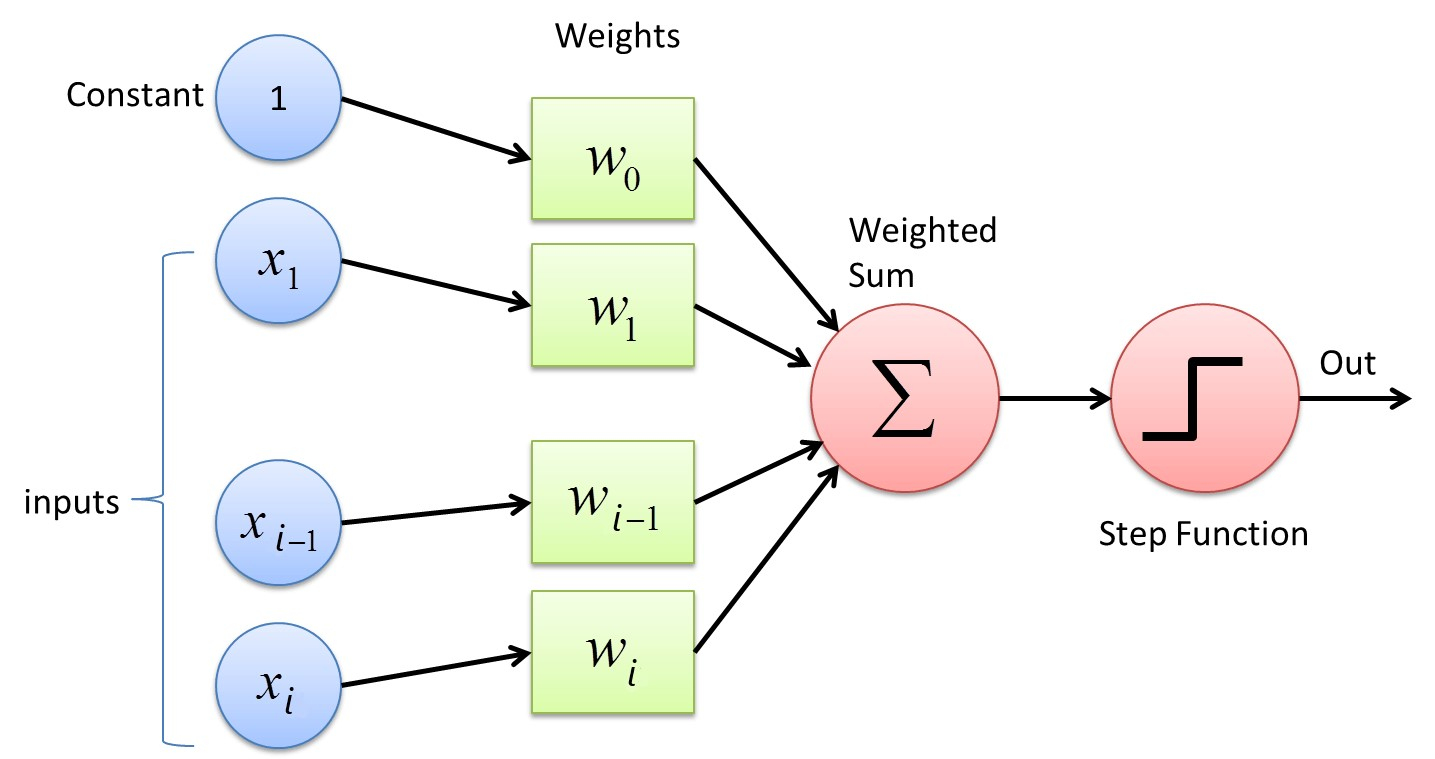
\includegraphics{images/Perceptron.jpg}
\caption{Schematic diagram of a perceptron.}\label{fig:Perceptron}
}
\end{figure}

(\url{https://images.deepai.org/glossary-terms/perceptron-6168423.jpg})

The perceptron can also be represented as a function. Analogous to the
representation above, the inputs \(x_{i}\) are multiplied by the weights
\(w_{i}\) in a linear combination. Then an error term is added so that
the whole can be packed into the non-linear activation function \(g(S)\)
. \(\hat{y}\) is the binary output of this perceptron.

\begin{align} \label{eq:perceptron}
\hat{y}=g(w_{0}+\sum_{i=1}^{n}x_{i}w_{i})
\end{align}

(Anthony and Bartlett, 1999)

The aim is to feed the perceptron with the training set and change the
weights \(w_{i}\) with each cycle so that the prediction becomes
accurate. The output value is compared to the desired value. Finally,
the sign of the difference \(y-\hat{y}\) determines whether the inputs
of that iteration are added to or subtracted from the weights. Ideally,
the weights will gradually converge and provide us with an usable model.

\hypertarget{multi-layer-perceptron}{%
\subsubsection{3.3. Multi layer
perceptron}\label{multi-layer-perceptron}}

Long-short-term-memory / Recurrent Neural Networks

Explain.

\hypertarget{bitcoin}{%
\subsubsection{3.3. Bitcoin}\label{bitcoin}}

In this section bitcoin as a cryptocurreny is introduced. The historical
data is analyzed and commentend. Further the technology around
cryptocurrencies is briefly explained. A detailed explanation would
requiere a paper itself, therefore the explantion is done as simple as
possible.

In the following work bitcoin as a cryptocurreny is mentionend in its
short term BTC, by the meaning of US Dollars per Bitcoin.

\hypertarget{historical-analysis}{%
\paragraph{3.3.1. Historical analysis}\label{historical-analysis}}

Bitcoin was first introduced in 2009 as the leader of a new era of
cryptocurrencies. Firstly the recognition wasnt very high due to the
fact of a non established technology. At the end of 2016 things began to
change, more volume was flushed in the market and the price of BTC began
to slowly ascend. in 2017 the real rally began and the BTC rose up to
nearly 20k USD / BTC. In the following years until 2020 BTC had a lot of
different phases from rising and falling to a price at the end in 2020
around 100 USD per BTC. Most recent events topped everything before, as
the BTC rose up to 58000 US Dollar after companies like Tesla and Signal
bougth in with high volume.

\begin{center}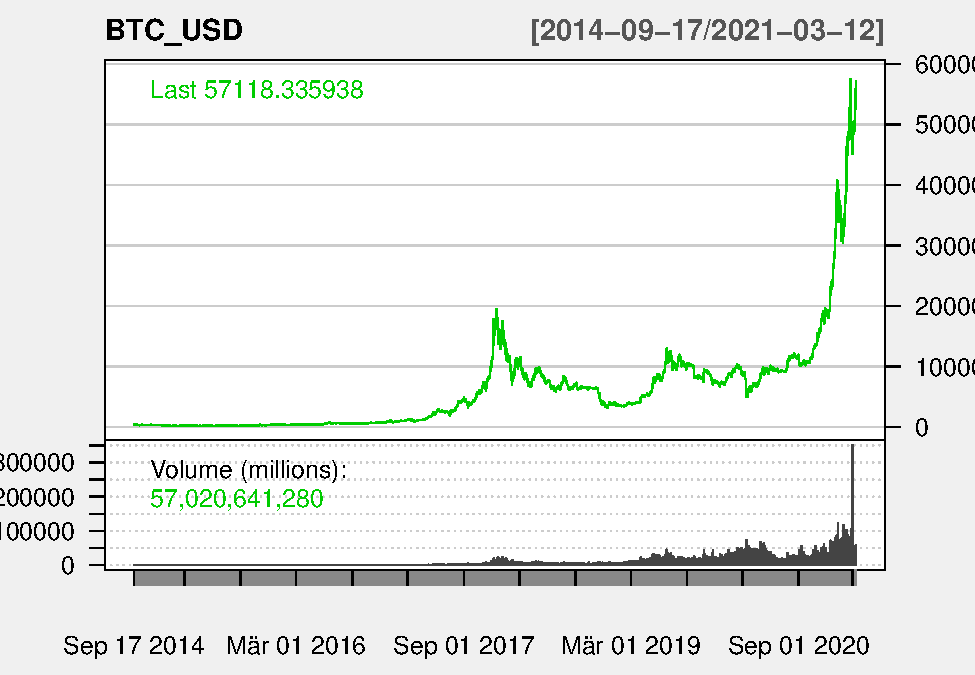
\includegraphics[width=0.7\linewidth]{00_main_files/figure-latex/unnamed-chunk-10-1} \end{center}

\hypertarget{sha256-hash}{%
\paragraph{3.3.2. SHA256 Hash}\label{sha256-hash}}

\begin{itemize}
\tightlist
\item
  Block
\item
  Blockchain
\item
  Distributed Blockchain
\item
  Token
\item
  Coinbase Transaction
\item
  Public/Private Key -\textgreater{} Signing
\item
  Signature (sign, verify)
\item
  Transaction
\end{itemize}

\newpage

\hypertarget{reference}{%
\subsubsection{3.7. Reference}\label{reference}}

\hypertarget{figure-reference}{%
\paragraph{3.7.1. Figure Reference}\label{figure-reference}}

~

As you can see in figure \ref{fig:fig1} -\textgreater{} GOOGLE

\begin{figure}

{\centering 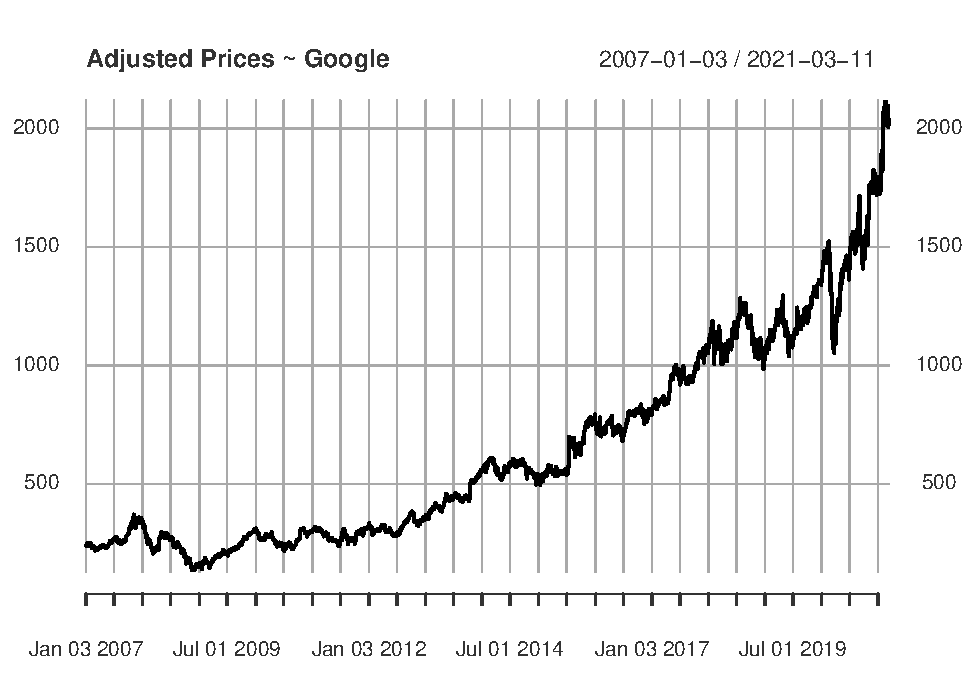
\includegraphics[width=0.7\linewidth]{00_main_files/figure-latex/fig1-1} 

}

\caption{Visualization of the adjusted prices of the Alphabet Inc Class A Stock.}\label{fig:fig1}
\end{figure}

\newpage

\hypertarget{equation-reference}{%
\paragraph{3.7.2. Equation Reference}\label{equation-reference}}

~

GARCH-formula can be seen in \ref{eq:garch}

\begin{align} \label{eq:garch}
  \epsilon_{t} &= \mathrm{log}(x_{t})-\mathrm{log}(x_{t-1}) \nonumber \\
  \epsilon_{t} &= \sigma_{t}u_{t} \\
  \sigma_{t}^{2} &=c \sigma^{2}+\sum_{j=1}^{n}\alpha_{j}\sigma_{t-j}^{2}+\sum_{k=1}^{m}\beta_{k}\epsilon_{t-k}^{2} \nonumber
\end{align}

\newpage

\hypertarget{table-reference}{%
\paragraph{3.7.3. Table Reference}\label{table-reference}}

~

In table \ref{tab:coeftable} you can see the flexerino of the
coefficients.

\begin{table}

\caption{\label{tab:coeftable}Coefficients GARCH(1,1).}
\centering
\begin{tabular}[t]{lrrr}
\toprule
  & Estimate & Std. Error & p-Value\\
\midrule
$\omega$ & 1.103223e-05 & 1.862651e-06 & 3.163846e-09\\
$\alpha_{1}$ & 7.386805e-02 & 1.075535e-02 & 6.509460e-12\\
$\beta_{1}$ & 8.943973e-01 & 1.381158e-02 & 0.000000e+00\\
\bottomrule
\end{tabular}
\end{table}

\newpage

\hypertarget{sec-ref}{%
\paragraph{3.7.4. Section Reference}\label{sec-ref}}

Here we can see a wild section, which will reference to itself:
\protect\hyperlink{sec-ref}{2.7.4.}

Or reference to the Bitcoin-section \protect\hyperlink{bitcoin}{2.3.}

\newpage

\hypertarget{literature-reference}{%
\paragraph{3.7.5. Literature Reference}\label{literature-reference}}

Add bibliography reference in the \texttt{.bib}-file in the add folder.

Here I make a reference to the original bitcoinpaper {[}1{]}
\texttt{{[}@bitcoin{]}} or to the specific page on the NN financial
trading paper {[}2, pp. 6--8{]} -\textgreater{}
\texttt{{[}@nnfin,\ pp.\ 6-8{]}}

\newpage

\hypertarget{methodology}{%
\subsection{4. Methodology}\label{methodology}}

The focus of this thesis is to predict historical prices of bitcoin
using the models listed in Chapter XX. The predictive accuracy of these
obtained predictions are compared using loss functions (Annualized
Sharpe, Diebold Mariano Test, MAE, MSE, RMSE, Mincer-Zarnowitz
Regressions). Then, based on the best models with the most accurate
predictions, trading strategies are worked out to compare with a
buy-and-hold strategy. Finally, we would like to venture into the topic
of explainability and attempt to explain why the chosen models lead to
these outcomes. The procedure of this quantitative study is described in
this chapter.

\begin{itemize}
\tightlist
\item
  Data and Analysis of Bitcoin (BTC/USD)
\item
  Defining the train and test samples (including description about calm
  and volatile phases).
\item
  Calculate predictions with the defined models (AR, NN, RNN, LSTM).
\item
  Compare Predictions with Realized Data (Annualized Sharpe, Diebold
  Mariano Test, MAE, MSE, RMSE, Mincer-Zarnowitz Regressions)
\item
  Explain trading strategies
\item
  Explainability for the best models
\item
  (Backup: Which models work well in which market phases?)
\end{itemize}

\hypertarget{data-and-analysis-of-bitcoin}{%
\subsubsection{4.1. Data and analysis of
Bitcoin}\label{data-and-analysis-of-bitcoin}}

\begin{itemize}
\item
  Source
\item
  Structure of data (intraday, daily etc.)
\item
  Why BTC/USD
\item
  Derivation of log-returns
\item
  Description of data (mean, sd, skewness, kurtosis, ADF)
\end{itemize}

\hypertarget{defining-train-and-test-samples}{%
\subsubsection{4.2. Defining train and test
samples}\label{defining-train-and-test-samples}}

\begin{itemize}
\item
  Describe different phases
\item
  Explain why we set train and test sample like this
\item
  Describe stable and volatile phases and why we should keep that in
  mind for predictions
\end{itemize}

\hypertarget{forecasting}{%
\subsubsection{4.3. Forecasting}\label{forecasting}}

\begin{itemize}
\item
  Autoregressive process (AR)
\item
  Deep learning neural network / multi layer percepton
\item
  Recurrent neural network (RNN)
\item
  Long short-term memory (LSTM)
\end{itemize}

\hypertarget{in-sample}{%
\subsubsection{4.3.1. In-sample}\label{in-sample}}

\begin{itemize}
\tightlist
\item
  Compare Predictions with Realized Data (Annualized Sharpe, Diebold
  Mariano Test, MAE, MSE, RMSE, Mincer-Zarnowitz Regressions)
\end{itemize}

\hypertarget{out-of-sample}{%
\subsubsection{4.3.2. Out-of-sample}\label{out-of-sample}}

\begin{itemize}
\tightlist
\item
  Compare Predictions with Realized Data (Annualized Sharpe, Diebold
  Mariano Test, MAE, MSE, RMSE, Mincer-Zarnowitz Regressions)
\end{itemize}

\hypertarget{trading-strategies}{%
\subsubsection{4.4. Trading strategies}\label{trading-strategies}}

\begin{itemize}
\item
  Define trading strategies
\item
  Define realistic fee structure for trading (Coinbase Pro, Binance,
  Kraken etc.)
\end{itemize}

\hypertarget{explainability}{%
\subsubsection{4.5. Explainability}\label{explainability}}

\begin{itemize}
\item
  Performing the predictions with the two (?) best models
\item
  Include variations to find possible starting points for explainability
  (number of nodes, layers)
\end{itemize}

\hypertarget{relationship-between-accuracy-and-market-phase}{%
\subsubsection{4.6. (Relationship between accuracy and market
phase)}\label{relationship-between-accuracy-and-market-phase}}

\begin{itemize}
\tightlist
\item
  Test
\end{itemize}

\newpage

\hypertarget{results}{%
\subsection{4. Results}\label{results}}

Lorem ipsum dolor sit amet, consectetur adipiscing elit, sed do eiusmod
tempor incididunt ut labore et dolore magna aliqua. Commodo elit at
imperdiet dui accumsan sit. Tempus iaculis urna id volutpat lacus
laoreet non curabitur gravida. Turpis egestas integer eget aliquet nibh
praesent tristique magna. Nec ultrices dui sapien eget mi proin sed.
Turpis nunc eget lorem dolor sed viverra ipsum nunc. Lorem donec massa
sapien faucibus et. In hac habitasse platea dictumst vestibulum rhoncus
est pellentesque. Ac tortor vitae purus faucibus ornare suspendisse sed
nisi lacus. Mauris cursus mattis molestie a iaculis at erat pellentesque
adipiscing.

\hypertarget{dummy-title-3}{%
\subsubsection{4.1. Dummy-Title}\label{dummy-title-3}}

Neque volutpat ac tincidunt vitae semper quis. At elementum eu facilisis
sed odio morbi quis commodo odio. Eget dolor morbi non arcu risus quis.
Gravida quis blandit turpis cursus in hac. Vehicula ipsum a arcu cursus
vitae congue mauris. Id eu nisl nunc mi ipsum faucibus vitae. Ut sem
viverra aliquet eget sit amet. Tempor orci eu lobortis elementum. Eu
feugiat pretium nibh ipsum consequat nisl vel pretium. Vel turpis nunc
eget lorem dolor sed viverra. Enim neque volutpat ac tincidunt. Eget
nullam non nisi est sit amet facilisis magna. Adipiscing commodo elit at
imperdiet dui accumsan sit amet. Diam vel quam elementum pulvinar etiam
non. In hac habitasse platea dictumst vestibulum rhoncus. Mattis aliquam
faucibus purus in massa. Netus et malesuada fames ac. In fermentum
posuere urna nec tincidunt praesent. Dolor sit amet consectetur
adipiscing. At in tellus integer feugiat scelerisque.

Tellus at urna condimentum mattis pellentesque id nibh. Morbi tempus
iaculis urna id volutpat lacus laoreet. Sem fringilla ut morbi tincidunt
augue interdum. Mauris nunc congue nisi vitae. Diam maecenas ultricies
mi eget. Vel quam elementum pulvinar etiam. Aliquam faucibus purus in
massa. In est ante in nibh mauris cursus. Non diam phasellus vestibulum
lorem sed risus ultricies. Sed vulputate mi sit amet mauris commodo quis
imperdiet massa. Lectus vestibulum mattis ullamcorper velit sed
ullamcorper morbi tincidunt ornare. Pellentesque habitant morbi
tristique senectus et netus et malesuada fames. Elit duis tristique
sollicitudin nibh sit amet commodo. A iaculis at erat pellentesque
adipiscing commodo elit. Quam viverra orci sagittis eu volutpat odio
facilisis. Eros donec ac odio tempor orci dapibus ultrices in iaculis.

\hypertarget{dummy-title-4}{%
\subsubsection{4.2. Dummy-Title}\label{dummy-title-4}}

Dui id ornare arcu odio ut sem nulla. Quam nulla porttitor massa id
neque aliquam vestibulum morbi. Nulla at volutpat diam ut venenatis.
Diam in arcu cursus euismod quis viverra nibh cras pulvinar.
Pellentesque pulvinar pellentesque habitant morbi tristique senectus et
netus. Posuere lorem ipsum dolor sit. Mus mauris vitae ultricies leo
integer malesuada nunc. Lorem donec massa sapien faucibus et molestie ac
feugiat. Erat pellentesque adipiscing commodo elit at imperdiet dui. Id
diam maecenas ultricies mi eget. Dui ut ornare lectus sit amet est
placerat in egestas. Commodo sed egestas egestas fringilla phasellus
faucibus scelerisque eleifend. Morbi blandit cursus risus at ultrices
mi. Mollis nunc sed id semper risus. Egestas sed sed risus pretium quam
vulputate dignissim suspendisse in. Vitae justo eget magna fermentum
iaculis. Pellentesque pulvinar pellentesque habitant morbi tristique.
Pharetra magna ac placerat vestibulum lectus. In hac habitasse platea
dictumst quisque sagittis. Sapien nec sagittis aliquam malesuada
bibendum arcu vitae elementum curabitur.

\hypertarget{dummy-title-5}{%
\subsubsection{4.2.1. Dummy-Title}\label{dummy-title-5}}

Velit euismod in pellentesque massa placerat duis ultricies lacus.
Senectus et netus et malesuada fames. Fringilla ut morbi tincidunt augue
interdum velit. Faucibus scelerisque eleifend donec pretium vulputate
sapien nec sagittis aliquam. Duis at consectetur lorem donec massa
sapien faucibus et. Lacus luctus accumsan tortor posuere ac. Nunc id
cursus metus aliquam eleifend mi in nulla. Quis risus sed vulputate odio
ut enim blandit. Ullamcorper eget nulla facilisi etiam dignissim diam
quis enim. Commodo ullamcorper a lacus vestibulum sed arcu non. Sit amet
commodo nulla facilisi nullam vehicula ipsum. Risus quis varius quam
quisque. Velit egestas dui id ornare arcu odio ut sem nulla. At in
tellus integer feugiat scelerisque varius morbi enim. Pharetra magna ac
placerat vestibulum lectus mauris ultrices eros in.

Magnis dis parturient montes nascetur ridiculus mus mauris vitae
ultricies. Viverra suspendisse potenti nullam ac tortor vitae purus
faucibus ornare. Eget gravida cum sociis natoque penatibus et magnis dis
parturient. Sit amet porttitor eget dolor morbi non arcu risus quis.
Fermentum et sollicitudin ac orci phasellus egestas tellus. Risus
viverra adipiscing at in tellus integer feugiat scelerisque. Pulvinar
pellentesque habitant morbi tristique senectus et netus. Lacus sed
viverra tellus in. Massa sed elementum tempus egestas sed. Euismod
lacinia at quis risus sed vulputate odio ut. Sed libero enim sed
faucibus. Tempor orci eu lobortis elementum.

\newpage

\hypertarget{conclusion}{%
\subsection{5. Conclusion}\label{conclusion}}

Best Trading Algorithm ever!

\hypertarget{get-rich-or-die-tryin}{%
\subsubsection{5.1. Get rich or die tryin}\label{get-rich-or-die-tryin}}

Neque volutpat ac tincidunt vitae semper quis. At elementum eu facilisis
sed odio morbi quis commodo odio. Eget dolor

\hypertarget{be-gme-stock-or-not-to-be-gme-stock}{%
\subsubsection{5.2. Be GME stock, or not to be GME
stock}\label{be-gme-stock-or-not-to-be-gme-stock}}

Tellus at urna condimentum mattis pellentesque id nibh. Morbi tempus
iaculis urna id volutpat lacus laoreet. Sem fringilla

\newpage

\hypertarget{references}{%
\subsection{5. References}\label{references}}

\hypertarget{refs}{}
\begin{CSLReferences}{0}{0}
\leavevmode\hypertarget{ref-bitcoin}{}%
\CSLLeftMargin{{[}1{]} }
\CSLRightInline{S. Nakamoto, \emph{Bitcoin: A peer-to-peer electronic
cash system}. online: www.bitcoin.org, 2008, p. 9.}

\leavevmode\hypertarget{ref-nnfin}{}%
\CSLLeftMargin{{[}2{]} }
\CSLRightInline{R. R. Georgios Sermpinis Andreas Karathanasopoulos,
\emph{Neural networks in financial trading}. online: Springer
Science+Business Media, 2019, p. 16.}

\end{CSLReferences}

\newpage

\hypertarget{attachment}{%
\subsection{6. Attachment}\label{attachment}}

This project work is created with R-4.0.2 , RStudio Version 1.4.904 and
RMarkdown in collaborative working via Git / Github

\end{document}
